% Options for packages loaded elsewhere
% Options for packages loaded elsewhere
\PassOptionsToPackage{unicode}{hyperref}
\PassOptionsToPackage{hyphens}{url}
\PassOptionsToPackage{dvipsnames,svgnames,x11names}{xcolor}
%
\documentclass[
  number,
  preprint]{elsarticle}
\usepackage{xcolor}
\usepackage[margin=0.75in]{geometry}
\usepackage{amsmath,amssymb}
\setcounter{secnumdepth}{5}
\usepackage{iftex}
\ifPDFTeX
  \usepackage[T1]{fontenc}
  \usepackage[utf8]{inputenc}
  \usepackage{textcomp} % provide euro and other symbols
\else % if luatex or xetex
  \usepackage{unicode-math} % this also loads fontspec
  \defaultfontfeatures{Scale=MatchLowercase}
  \defaultfontfeatures[\rmfamily]{Ligatures=TeX,Scale=1}
\fi
\usepackage{lmodern}
\ifPDFTeX\else
  % xetex/luatex font selection
\fi
% Use upquote if available, for straight quotes in verbatim environments
\IfFileExists{upquote.sty}{\usepackage{upquote}}{}
\IfFileExists{microtype.sty}{% use microtype if available
  \usepackage[]{microtype}
  \UseMicrotypeSet[protrusion]{basicmath} % disable protrusion for tt fonts
}{}
\makeatletter
\@ifundefined{KOMAClassName}{% if non-KOMA class
  \IfFileExists{parskip.sty}{%
    \usepackage{parskip}
  }{% else
    \setlength{\parindent}{0pt}
    \setlength{\parskip}{6pt plus 2pt minus 1pt}}
}{% if KOMA class
  \KOMAoptions{parskip=half}}
\makeatother
% Make \paragraph and \subparagraph free-standing
\makeatletter
\ifx\paragraph\undefined\else
  \let\oldparagraph\paragraph
  \renewcommand{\paragraph}{
    \@ifstar
      \xxxParagraphStar
      \xxxParagraphNoStar
  }
  \newcommand{\xxxParagraphStar}[1]{\oldparagraph*{#1}\mbox{}}
  \newcommand{\xxxParagraphNoStar}[1]{\oldparagraph{#1}\mbox{}}
\fi
\ifx\subparagraph\undefined\else
  \let\oldsubparagraph\subparagraph
  \renewcommand{\subparagraph}{
    \@ifstar
      \xxxSubParagraphStar
      \xxxSubParagraphNoStar
  }
  \newcommand{\xxxSubParagraphStar}[1]{\oldsubparagraph*{#1}\mbox{}}
  \newcommand{\xxxSubParagraphNoStar}[1]{\oldsubparagraph{#1}\mbox{}}
\fi
\makeatother


\usepackage{longtable,booktabs,array}
\newcounter{none} % for unnumbered tables
\usepackage{calc} % for calculating minipage widths
% Correct order of tables after \paragraph or \subparagraph
\usepackage{etoolbox}
\makeatletter
\patchcmd\longtable{\par}{\if@noskipsec\mbox{}\fi\par}{}{}
\makeatother
% Allow footnotes in longtable head/foot
\IfFileExists{footnotehyper.sty}{\usepackage{footnotehyper}}{\usepackage{footnote}}
\makesavenoteenv{longtable}
\usepackage{graphicx}
\makeatletter
\newsavebox\pandoc@box
\newcommand*\pandocbounded[1]{% scales image to fit in text height/width
  \sbox\pandoc@box{#1}%
  \Gscale@div\@tempa{\textheight}{\dimexpr\ht\pandoc@box+\dp\pandoc@box\relax}%
  \Gscale@div\@tempb{\linewidth}{\wd\pandoc@box}%
  \ifdim\@tempb\p@<\@tempa\p@\let\@tempa\@tempb\fi% select the smaller of both
  \ifdim\@tempa\p@<\p@\scalebox{\@tempa}{\usebox\pandoc@box}%
  \else\usebox{\pandoc@box}%
  \fi%
}
% Set default figure placement to htbp
\def\fps@figure{htbp}
\makeatother





\setlength{\emergencystretch}{3em} % prevent overfull lines

\providecommand{\tightlist}{%
  \setlength{\itemsep}{0pt}\setlength{\parskip}{0pt}}



 
\usepackage[]{natbib}
\bibliographystyle{elsarticle-num}


\makeatletter
\@ifpackageloaded{caption}{}{\usepackage{caption}}
\AtBeginDocument{%
\ifdefined\contentsname
  \renewcommand*\contentsname{Table of contents}
\else
  \newcommand\contentsname{Table of contents}
\fi
\ifdefined\listfigurename
  \renewcommand*\listfigurename{List of Figures}
\else
  \newcommand\listfigurename{List of Figures}
\fi
\ifdefined\listtablename
  \renewcommand*\listtablename{List of Tables}
\else
  \newcommand\listtablename{List of Tables}
\fi
\ifdefined\figurename
  \renewcommand*\figurename{Figure}
\else
  \newcommand\figurename{Figure}
\fi
\ifdefined\tablename
  \renewcommand*\tablename{Table}
\else
  \newcommand\tablename{Table}
\fi
}
\@ifpackageloaded{float}{}{\usepackage{float}}
\floatstyle{ruled}
\@ifundefined{c@chapter}{\newfloat{codelisting}{h}{lop}}{\newfloat{codelisting}{h}{lop}[chapter]}
\floatname{codelisting}{Listing}
\newcommand*\listoflistings{\listof{codelisting}{List of Listings}}
\makeatother
\makeatletter
\makeatother
\makeatletter
\@ifpackageloaded{caption}{}{\usepackage{caption}}
\@ifpackageloaded{subcaption}{}{\usepackage{subcaption}}
\makeatother
\journal{Template Journal}
\usepackage{bookmark}
\IfFileExists{xurl.sty}{\usepackage{xurl}}{} % add URL line breaks if available
\urlstyle{same}
\hypersetup{
  pdftitle={GNC Assignment: Solution Approach},
  pdfauthor={Kiran M Aralikatti},
  colorlinks=true,
  linkcolor={blue},
  filecolor={Maroon},
  citecolor={Blue},
  urlcolor={Blue},
  pdfcreator={LaTeX via pandoc}}


\setlength{\parindent}{6pt}
\begin{document}

\begin{frontmatter}
\title{GNC Assignment: Solution Approach \\\large{Bellatrix Aerospace
Pvt. Ltd} }
\author[]{Kiran M Aralikatti%
%
}





        





\end{frontmatter}
    

\section{Introduction}\label{sec-introduction}

The document contains the various solution methods for the GNC
assignment problems. The given problems can be solved using more then
one method, which author tried to implement. The document generated
using \href{https://quarto.org/docs/journals/}{Quarto} locally, created
by the author. The source remains editable as a normal \texttt{.qmd}
manuscript and the template can be found
\href{https://github.com/kirancoder/paper_template/tree/main/sample_paper}{here}.

\section{Task 1}\label{sec-task1}

This is a very intersting geometery problem, which can solved using
trignometric relations to a triangles in a minor sector and also
converting the problem in polar co-ordinates.

The 1st and formost the cone has to opened and converted into a sector
of a circle, for a given right circular cone in the problem, it will
always be a minor sector of a circle. For both the methods, minor sector
will be used to find the downhill distance.

The 2nd catch is, when the cone is opened, the curve connecting point A
and B will be stright line, which is the shortest distance between two
points.

The below image shows the above discussed points, where the cone is
opened and the curve connecting A and B is stright line.

\begin{figure}[H]

\begin{minipage}[t]{0.50\linewidth}

\centering{

\pandocbounded{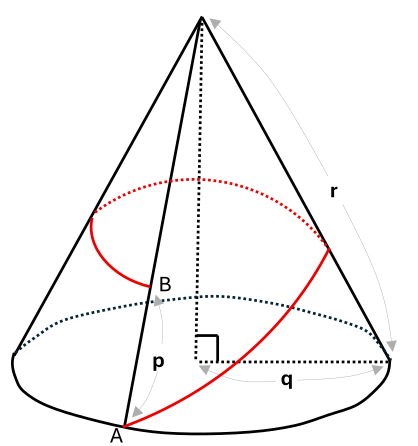
\includegraphics[keepaspectratio]{images/GNC_img_1.png}}

}

\subcaption{\label{fig-given-cone}}

\end{minipage}%
%
\begin{minipage}[t]{0.50\linewidth}

\centering{

\pandocbounded{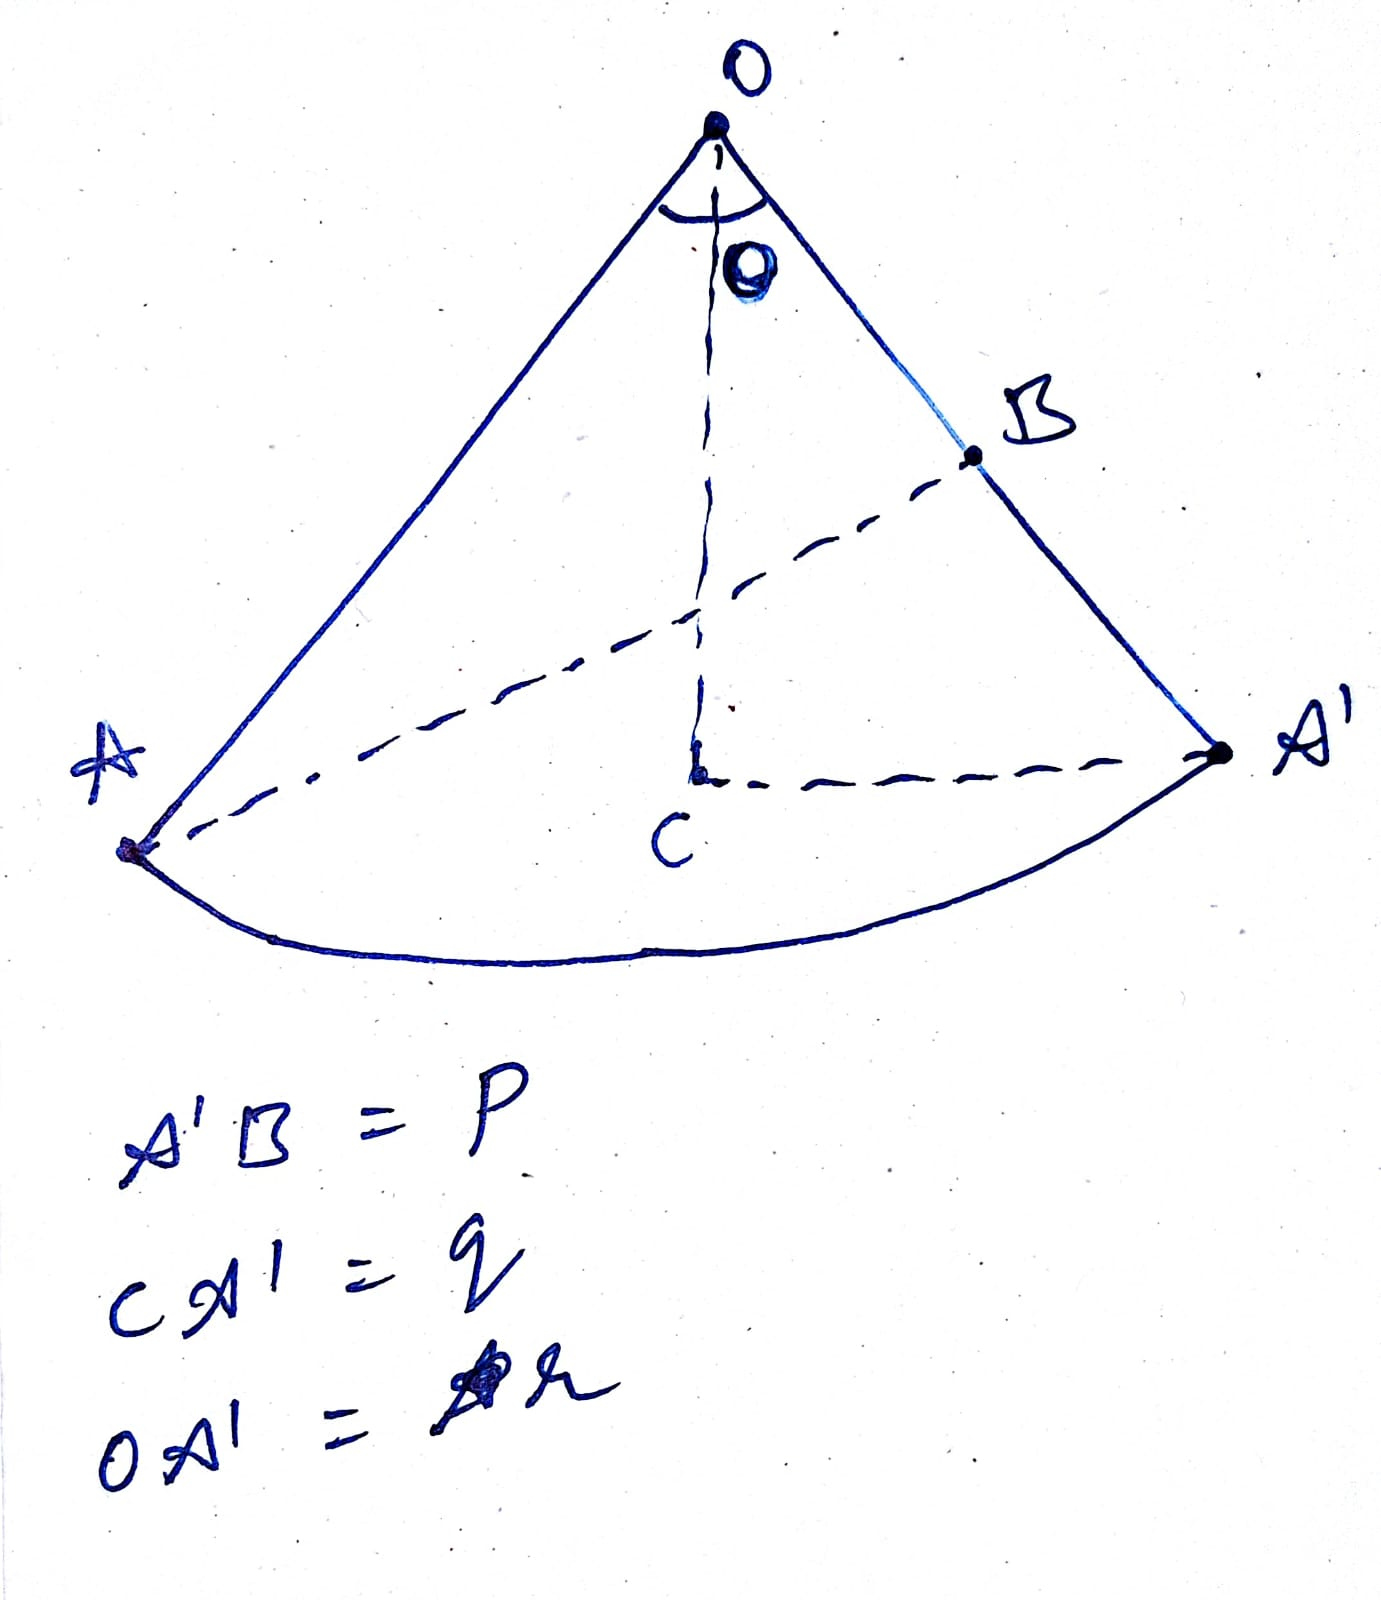
\includegraphics[keepaspectratio]{images/GNC_img_2.png}}

}

\subcaption{\label{fig-opened-cone}}

\end{minipage}%

\caption{\label{fig-cone}Given cone and its corresponding sector
representation.}

\end{figure}%

\subsection{Solution 1}\label{sec-task1-sol1}

In the given Figure~\ref{fig-opened-cone}, shows that the lengths of the
given cone ``p, q, r'' relation to the various lenths of the minor
sector.

Considering the person is going from the point A to B, the downhill
distance will lie on the somewhere on the line connecting A and B. The
distance can be calculated using trignometric relations to the triangle
\(\Delta \;ABO\) formed in the minor sector \(OAA'\).

To define the uphill while moving on the line AB, one can imgaine moving
closer to the point O, i.e.~and then moving away from the point O, until
reaching the point B. The divide the line segement AB into two parts,
uphill and downhill, we a need a point of AB, which lies close to the
point O, this can be found by draiwing a perpendicular from the point O
to the line AB, which will intersect at a point D. The point D will be
the closest point to O on the line AB, and hence the point D will be the
point where the uphill ends and downhill starts.

The below image will show the point D in the \(\Delta \;ABO\) triangle,
which is the closest point to O on the line AB.

\begin{figure}[H]

\begin{minipage}[t]{\linewidth}

\pandocbounded{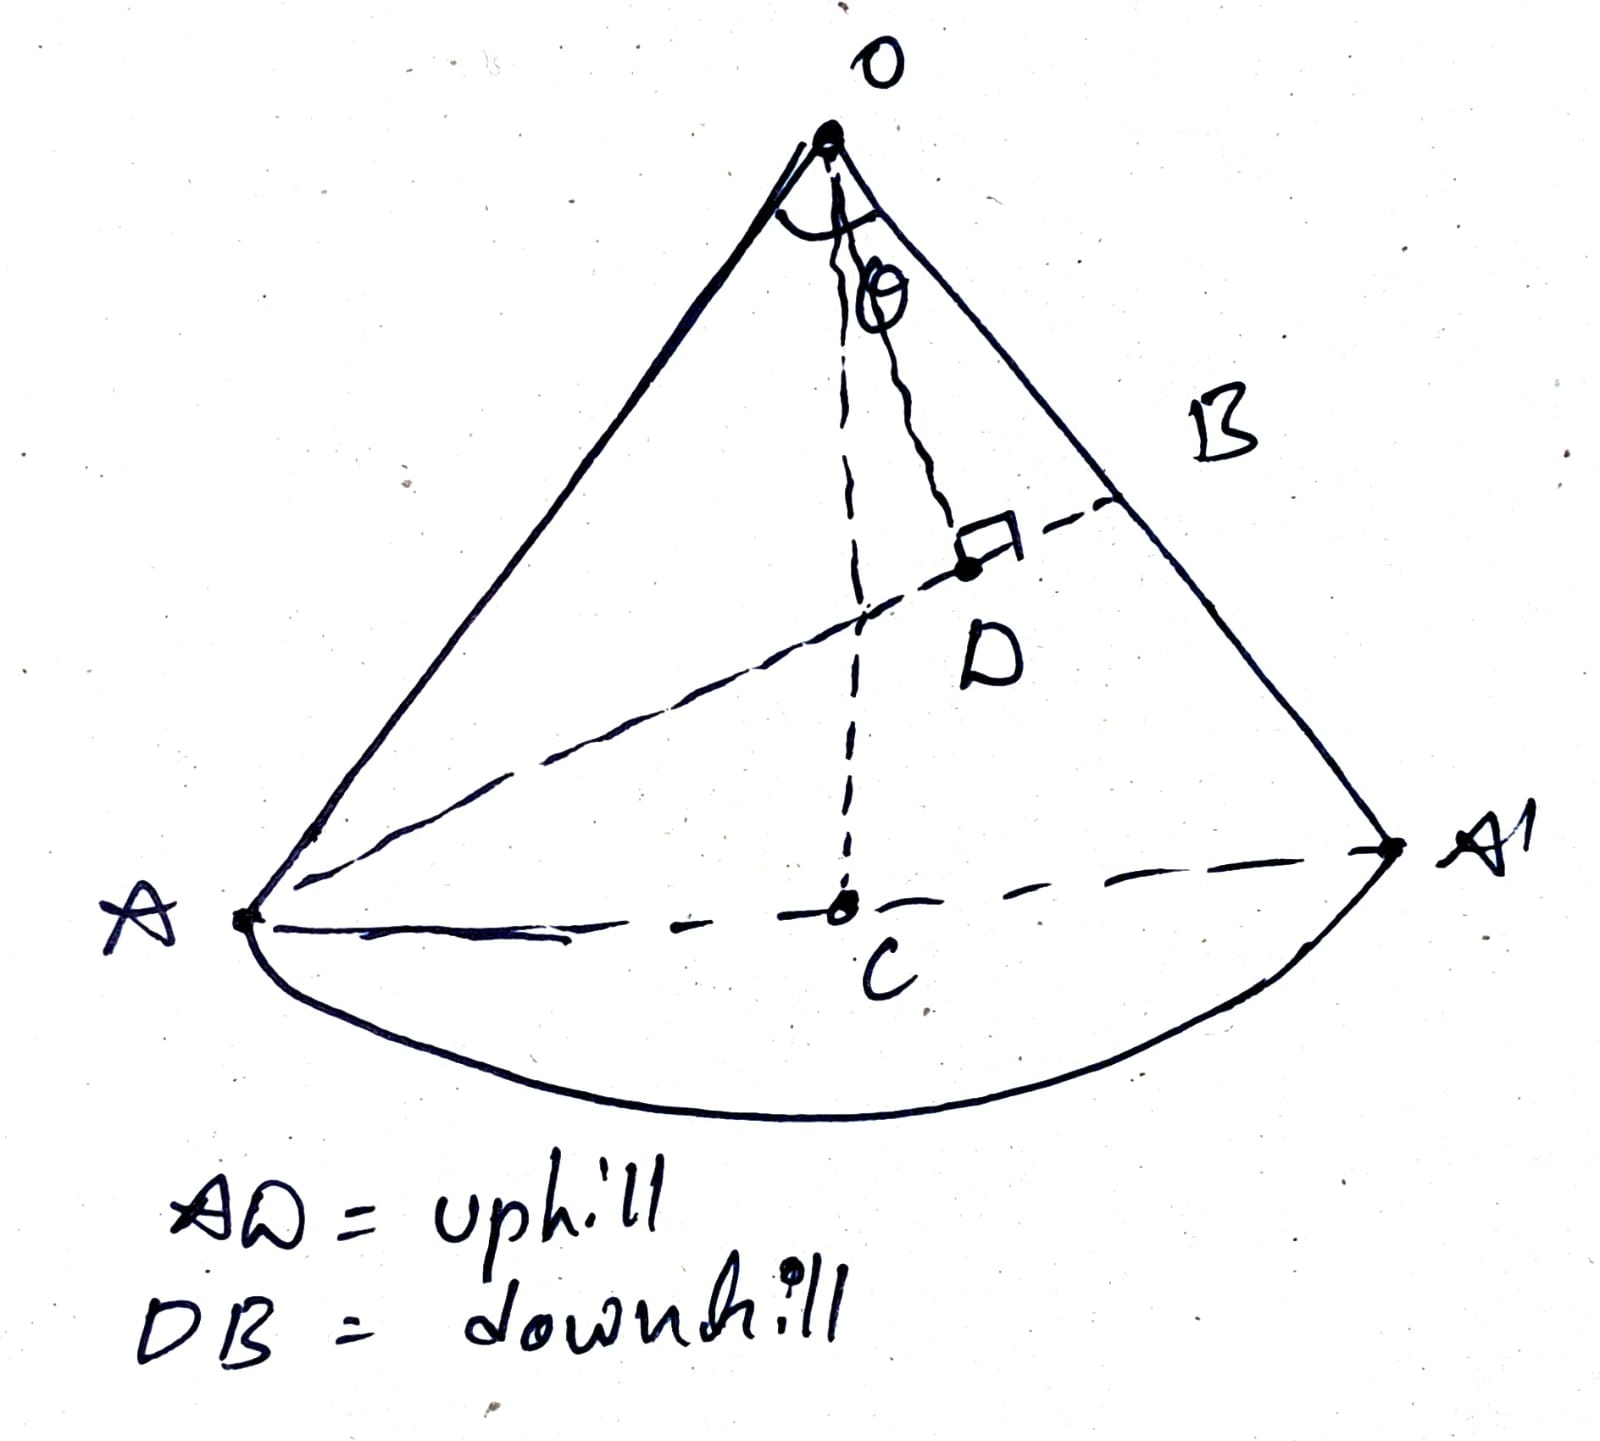
\includegraphics[keepaspectratio]{images/GNC_img_3.png}}

\end{minipage}%

\caption{\label{fig-cone}Representation of the uphill and downhill
paths.}

\end{figure}%

So the task is now to find the distance DB, as the function of the given
lengths p, q and r.

The \(\Delta \; ABO\) the \(\angle\; \theta\), is common between the
\(\Delta \; ABO\) and the sector. By the realtion between the angle and
arc in circle,
\begin{equation}\protect\phantomsection\label{eq-r_theta}{
\theta = \frac{l}{r}
}\end{equation}

where \(l = \overset{\frown}{AB}\) and \(r\) is radius and \(\theta\) is
angle suspended by the sector.

The lengths \(q\) which is the radius of the cone, the permeter of the
sector can derivied from that,
\begin{equation}\protect\phantomsection\label{eq-cone}{
\overset{\frown}{AB} = 2\, \pi \, q
}\end{equation}

Now, substiting arc length relation into Equation~\ref{eq-r_theta},

\[
\theta = \frac{2\, \pi \, q}{r}
\]

Hence, \(\theta  = f(q,r)\).

Now, in \(\Delta AOB\), and \(\theta\) and two sides (\(OA = r\) \&
\(OB = r - p\)) known in terms of the known quantites, so we can now
apply \(cosine\) rule to find the third side, \(AB\) in terms of given
parameters \(p, \; q \& r\)

\begin{equation}\protect\phantomsection\label{eq-cosine}{
{AB}^2 = {OA}^2 + {OB}^2 - 2 \cdot OA \cdot OB \; cos(\theta) = r^2+(r-p)^2-2r(r-p)\cos\theta
}\end{equation}

Consider \(AB = k\)

\[
k = \sqrt{r^2+(r-p)^2-2r(r-p)\cos\theta}
\]

Now, for the \(\Delta AOD\) and \(\Delta DOB\) are right angle
triangles, the side \(OD\):
\begin{equation}\protect\phantomsection\label{eq-tri-rel}{
\begin{aligned}
OD^2 = OA^2 - AD^2 \quad \text{in } \Delta AOD \\
OD^2 = OB^2 - BD^2 \quad \text{in } \Delta DOB
\end{aligned}
}\end{equation}

For simiplification consider \(AD = m \; \text{and} \; DB = n\) which is
line \(AB\) defined above, then from Equation~\ref{eq-tri-rel} \[
r^2 - m^2 = (r-p)^2 - n^2
\]

here \(m\) is uphill distance and \(n\) is downhill distance and
simplifying the above solution gives,
\begin{equation}\protect\phantomsection\label{eq-main}{
\begin{aligned}
m^2 - n^2 = r^2 - (r-p)^2 \\
(m+n)(m-n) = r^2 - (r-p)^2
\end{aligned}
}\end{equation}

then,

\begin{equation}\protect\phantomsection\label{eq-main-2}{
m-n = \frac{r^2 - (r-p)^2}{m+n} = \frac{r^2 - (r-p)^2}{k} 
}\end{equation}

and from the relations of \(k, m \; \text{and} \; n\),
\begin{equation}\protect\phantomsection\label{eq-main-1}{
m + n = k
}\end{equation}

Now, substract Equation~\ref{eq-main-2} from Equation~\ref{eq-main-1}
gives

\[
\begin{aligned}
2n = \frac{k^2 - r^2 + (r-p)^2}{k}
\end{aligned}
\]

Substitute the value of \(k\) and simplify,

\[
\begin{aligned}
n = \frac{(r-p)^2 - r(r-p) cos(\theta)}{\sqrt{r^2+(r-p)^2-2r(r-p)\cos\theta}}
\end{aligned}
\]

So, the downhill distance (\(n\)), is the function
\(p, q, \text{and} r\) as \(\theta\) is also function of
\(p, q, \; \text{and} \; r\)

\[
n = g(p, q, r)
\]

\pagebreak


\renewcommand\refname{References}
\bibliography{references.bib}



\end{document}
